\documentclass{beamer}

\usepackage[size=custom,width=91.44,height=121.92,orientation=portrait,scale=1.8]{beamerposter}
\usetheme{LLT-poster}
\usecolortheme{Entrepreneur}

\usepackage[utf8]{inputenc}
\usepackage[T1]{fontenc}
\usepackage{libertine}
\usepackage[scaled=0.92]{inconsolata}
\usepackage[libertine]{newtxmath}
\usepackage{wrapfig}
\usepackage{mathtools}
\usepackage{calc}
\usepackage{mwe}

\usepackage{hyperref}
\hypersetup{
    colorlinks=true,       % false: boxed links; true: colored links
    urlcolor=cyan           % color of external links
}

\usepackage{tikz}

\usepackage{xcolor}
\usepackage{listings}

\newcommand\JSONnumbervaluestyle{\color{blue}}
\newcommand\JSONstringvaluestyle{\color{blue}}

\newif\ifcolonfoundonthisline

\makeatletter

\lstdefinestyle{json}
{
  showstringspaces    = false,
  alsoletter          = 0123456789.,
  morestring          = [s]{"}{"},
  stringstyle         = \ifcolonfoundonthisline\JSONstringvaluestyle\fi,
  MoreSelectCharTable =%
    \lst@DefSaveDef{`:}\colon@json{\processColon@json},
  basicstyle          = \ttfamily\small,
  keywordstyle        = \ttfamily\bfseries,
}

\newcommand\processColon@json{%
  \colon@json%
  \ifnum\lst@mode=\lst@Pmode%
    \global\colonfoundonthislinetrue%
  \fi
}

\lst@AddToHook{Output}{%
  \ifcolonfoundonthisline%
    \ifnum\lst@mode=\lst@Pmode%
      \def\lst@thestyle{\JSONnumbervaluestyle}%
    \fi
  \fi
  \lsthk@DetectKeywords% 
}

\lst@AddToHook{EOL}%
  {\global\colonfoundonthislinefalse}


\usebackgroundtemplate{\tikz\node[opacity=0.1]{\includegraphics[width=\paperwidth,height=\paperheight]{img/world.png}};}

\title{\raisebox{\heightof{B)}-\height+7mm}{\includegraphics[height=1.3em]{img/logo.png}} Beacon: A Protocol for Federated Discovery and Sharing of Genomic Data}
\author[L. Dolman, I. Lappalainen, M. Linden, J. D. Spalding, A. Page, P. Flicek, S. Sherry, D. Haussler, Beacon Project Team]{M. Fiume, M. Cupak, S. Keenan, J. Rambla, S. O. M. Dyke, A. J. Brookes, K. Carey, D. Lloyd, P. Goodhand, M. Haeussler, M. Baudis,}
\footimage{\includegraphics[width=3.5em]{img/ga4gh.png}}

\begin{document}
\begin{frame}[fragile]

\begin{block}{Motivation\hfill\raisebox{\heightof{B)}-\height+2pt}{\includegraphics[height=1em]{img/idea.png}}}
\begin{itemize}
\item Analysis of large volumes of genomic data has the potential to drive discoveries and applications in medicine.
\item No institution has enough resources to capture all human variation.
\item Standards for interoperability enabling sharing across a federated network of genomic data resources are needed.
\end{itemize}
\end{block}
\vspace{-.5em}

\begin{columns}[T]
\begin{column}{.48\textwidth}

\begin{block}{Beacon\hfill\raisebox{\heightof{B)}-\height+2pt}{\includegraphics[height=1em]{img/logo.png}}}
\begin{itemize}
\item Standard defining a web service for discovery and sharing of information about alleles.
\item Demonstration of willingness of international organizations to share data.
\item Initiative of the Global Alliance for Genomics \& Health.
\item More information: \url{https://ga4gh.org/#/beacon}.
\end{itemize}
\end{block}

\begin{block}{API\hfill\raisebox{\heightof{B)}-\height+2pt}{\includegraphics[height=1em]{img/protocol.png}}}
\begin{itemize}
\item Request: \textit{"Do you have information about this mutation?"}.
\begin{lstlisting}[style=json]
{
  "referenceName": "13",
  "start": 32936731,
  "referenceBases": "G",
  "alternateBases": "C",
  "assemblyId": "GRCh37"
}
\end{lstlisting}
\item Response: \textit{"yes"}/\textit{"no"} (optionally additional information about the mutation).
\begin{lstlisting}[style=json]
{
  "exists": true,
  "datasetAlleleResponses":  [
    {
      "exists": true,
      "info": {
  ...
\end{lstlisting}
\item Supported by a variety of tools, e.g. reference implementation, command line client, query library, sample beacons in multiple programming languages, adapters for various sources of genomic data.
\item More information: \url{https://github.com/ga4gh/beacon-team}.
\end{itemize}
\end{block}

\begin{block}{Participants\hfill\raisebox{\heightof{B)}-\height+2pt}{\includegraphics[height=1em]{img/participants.png}}}
\begin{itemize}
\item 25+ of the world's top genomic organizations, 60+ beacons.

\vspace{2mm}
\begin{center}
\includegraphics[width=\linewidth]{img/map2.png}
\end{center}
\item 160+ datasets of various origins, e.g. sequence observations from patients, population studies, in-silico predictions, curated/crowd-sourced databases, scientific literature.
\end{itemize}
\end{block}
\end{column}


\begin{column}{.46\textwidth}
\begin{block}{Beacon Network\hfill\raisebox{\heightof{B)}-\height+2pt}{\includegraphics[height=1em]{img/beacon-network.png}}}
\begin{itemize}
\item Search engine across the world's beacons.

\vspace{2mm}
\begin{center}
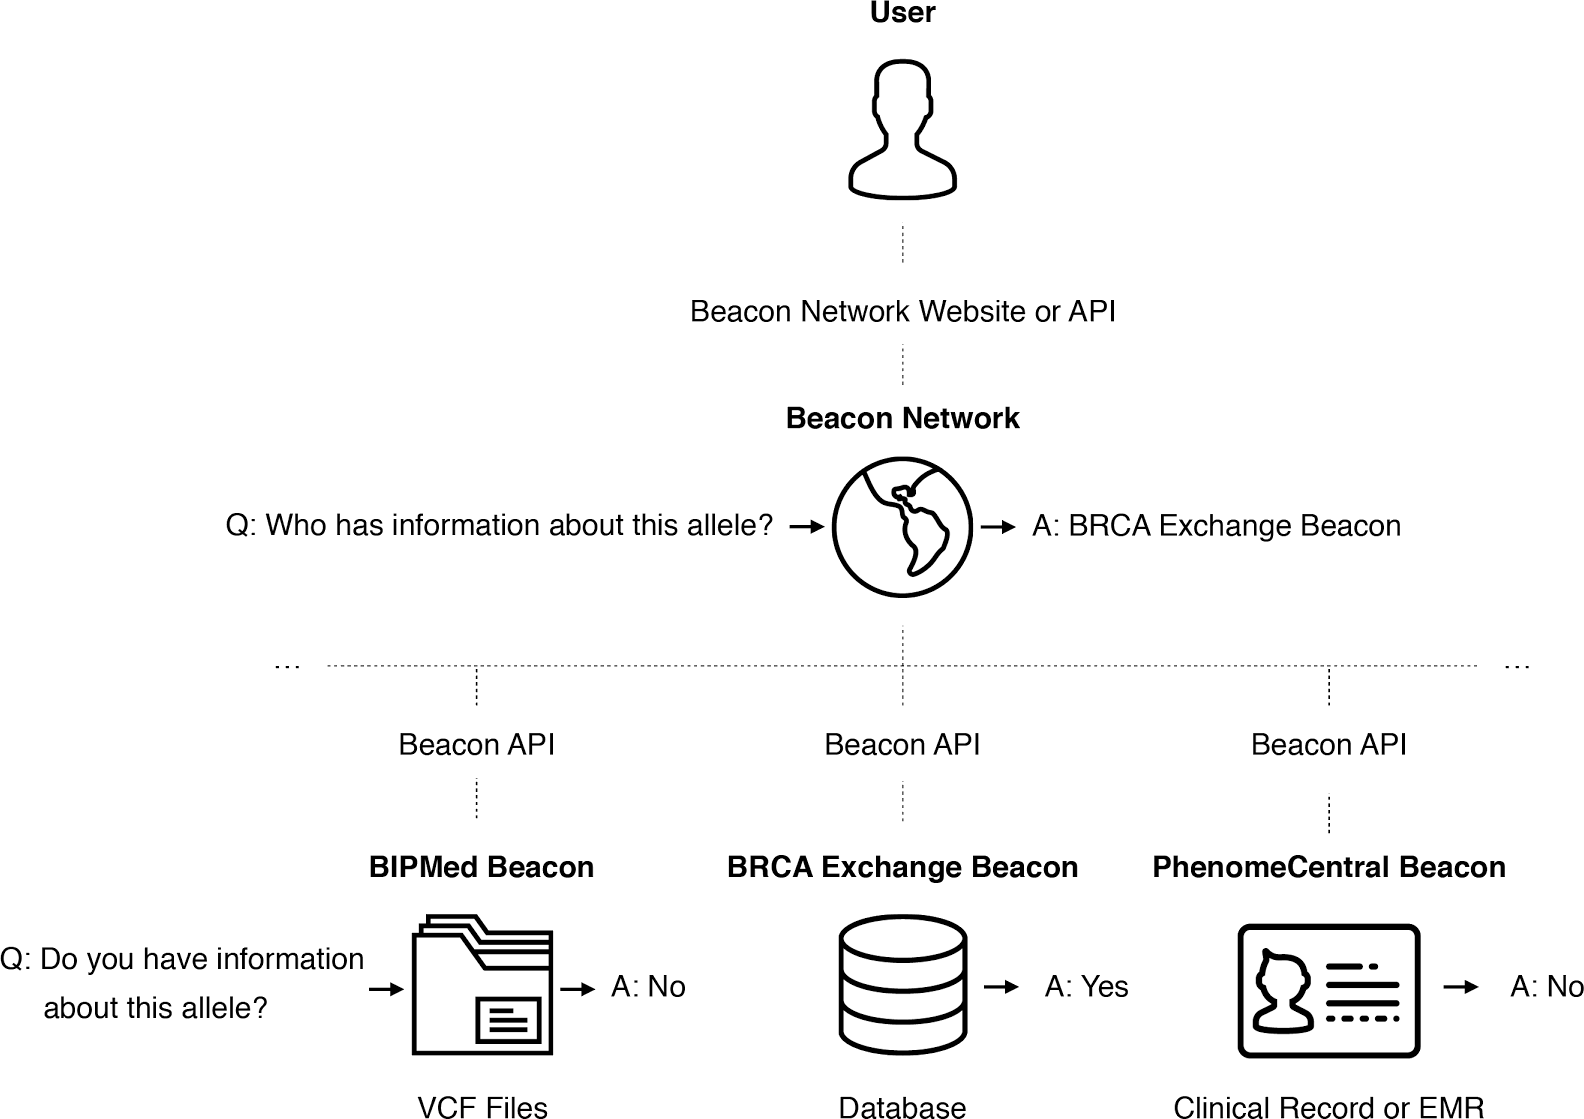
\includegraphics[width=\linewidth]{img/schema.png}
\end{center}
\item Translates genomic queries for each beacon, intelligently distributes the queries through the network, and aggregates the results.

\vspace{2mm}
\begin{center}
\includegraphics[width=\linewidth]{img/client.png}
\end{center}

\item Served 400K+ queries from 6K+ users in 100+ countries, resulting in 2M+ queries dispatched to the participants of the network.

\vspace{2mm}
\begin{center}
\includegraphics[width=\linewidth]{img/queries.png}
\end{center}

\item More information: \url{http://beacon-network.org}.
\end{itemize}
\end{block}
\end{column}

\end{columns}
\end{frame}
\end{document}